\section{Localizar mão de obra}

\par Uma das funcionalidades implementadas no desenvolvimento foi a busca por mão de obra. Esta busca permite que o usuário encontre profissionais que desempenham a função específica procurada por ele. Para realizar esta busca, foi preciso escrever uma consulta que leva em conta três níveis de análise, sendo elas, a busca pelo profissional que desempenha o trabalho dentro da rede de parceiros do usuário, dentro da empresa onde o ele trabalha e por último, dentro da cidade onde vive.  

\par Para escrever esta consulta foi utilizada a tecnologia \textit{Cypher}, que é uma linguagem específica para o banco Neo4j \cite{neo4j_team_manual}. O Código~\ref{list:consulta_busca} apresenta a \textit{query} utilizada para realizar esta busca.

% Alterado para listagem
%\newpage
%\begin{figure}[h!]
%	\centerline{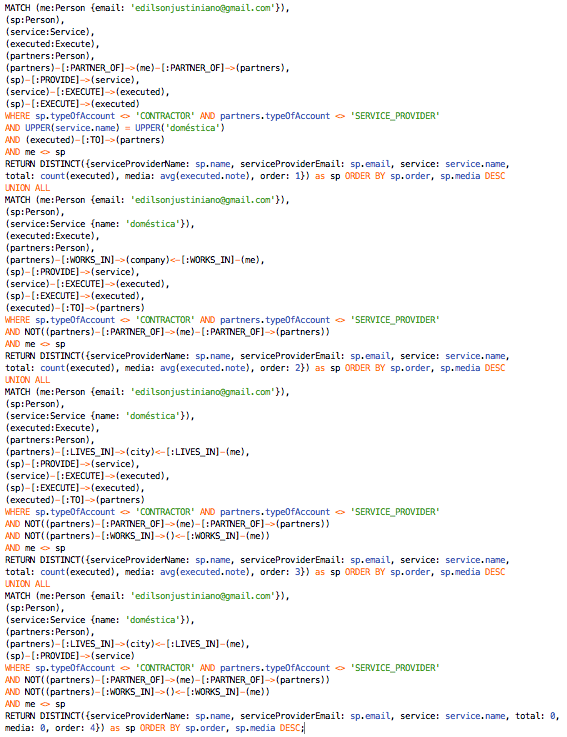
\includegraphics[scale=0.7]{./imagens/consulta-busca-domestica.png}}
%	\caption[\textit{Query} para localização de mão de obra.]
%	{\textit{Query} para localização de mão de obra \textbf{Fonte:} Elaborado pelos autores.}
%	\label{fig:consulta_busca}
%\end{figure}

\begin{lstlisting} [style=custom_SQL,caption={[\textit{Query} para localização de mão de obra]{\textit{Query} para localização de mão de obra. \textbf{Fonte:} Elaborado pelos autores.}}, label=list:consulta_busca] 	
MATCH (me:Person {email: 'edilsonjustiniano@gmail.com'}), (sp:Person), 
(service:Service), (executed:Execute), (partners:Person), 
(partners)-[:PARTNER_OF]->(me)-[:PARTNER_OF]->(partners),
(sp)-[:PROVIDE]->(service), (service)-[:EXECUTE]->(executed),
(sp)-[:EXECUTE]->(executed)
WHERE sp.typeOfAccount <> 'CONTRACTOR' 
AND partners.typeOfAccount <> 'SERVICE_PROVIDER'
AND UPPER(service.name) = UPPER('Domestica')
AND (executed)-[:TO]->(partners) AND me <> sp
RETURN DISTINCT({serviceProviderName: sp.name, 
serviceProviderEmail: sp.email, service: service.name,
total: count(executed), media: avg(executed.note), order: 1}) as sp 
ORDER BY sp.order, sp.media DESC
UNION ALL
MATCH (me:Person {email: 'edilsonjustiniano@gmail.com'}), (sp:Person),
(service:Service {name: 'Domestica'}), (executed:Execute),
(partners:Person), (partners)-[:WORKS_IN]->(company)<-[:WORKS_IN]-(me),
(sp)-[:PROVIDE]->(service), (service)-[:EXECUTE]->(executed), 
(sp)-[:EXECUTE]->(executed), (executed)-[:TO]->(partners)
WHERE sp.typeOfAccount <> 'CONTRACTOR' 
AND partners.typeOfAccount <> 'SERVICE_PROVIDER'
AND NOT((partners)-[:PARTNER_OF]->(me)-[:PARTNER_OF]->(partners))
AND me <> sp
RETURN DISTINCT({serviceProviderName: sp.name, 
serviceProviderEmail: sp.email, service: service.name, 
total: count(executed), media: avg(executed.note), order: 2}) as sp 
ORDER BY sp.order, sp.media DESC
UNION ALL
MATCH (me:Person {email: 'edilsonjustiniano@gmail.com'}), (sp:Person),
(service:Service {name: 'Domestica'}), (executed:Execute), 
(partners:Person), (partners)-[:LIVES_IN]->(city)<-[:LIVES_IN]-(me),
(sp)-[:PROVIDE]->(service), (service)-[:EXECUTE]->(executed), 
(sp)-[:EXECUTE]->(executed), (executed)-[:TO]->(partners)
WHERE sp.typeOfAccount <> 'CONTRACTOR' 
AND partners.typeOfAccount <> 'SERVICE_PROVIDER'
AND NOT((partners)-[:PARTNER_OF]->(me)-[:PARTNER_OF]->(partners))
AND NOT((partners)-[:WORKS_IN]->()<-[:WORKS_IN]-(me))
AND me <> sp
RETURN DISTINCT({serviceProviderName: sp.name, 
serviceProviderEmail: sp.email, service: service.name, 
total: count(executed), media: avg(executed.note), order: 3}) as sp 
ORDER BY sp.order, sp.media DESC 
UNION ALL
MATCH (me:Person {email: 'edilsonjustiniano@gmail.com'}), (sp:Person),
(service:Service {name: 'Domestica'}), (partners:Person),
(partners)-[:LIVES_IN]->(city)<-[:LIVES_IN]-(me), 
(sp)-[:PROVIDE]->(service)
WHERE sp.typeOfAccount <> 'CONTRACTOR' 
AND partners.typeOfAccount <> 'SERVICE_PROVIDER'
AND NOT((partners)-[:PARTNER_OF]->(me)-[:PARTNER_OF]->(partners))
AND NOT((partners)-[:WORKS_IN]->()<-[:WORKS_IN]-(me))
AND me <> sp
RETURN DISTINCT({serviceProviderName: sp.name, 
serviceProviderEmail: sp.email, service: service.name, total: 0,
media: 0, order: 4}) as sp ORDER BY sp.order, sp.media DESC;
\end{lstlisting}

Essa consulta é dividida em quatro sub consultas separadas pela cláusula \texttt{UNION ALL}, a fim de atingir um número maior de possibilidades de pestadores de serviços ao usuário, sendo que a primeira delas está recuperando os dados de pessoas que proveram o serviço de doméstica para usuários que possuem o relacionamento de parceria com o usuário autenticado no sistema, nesse caso o \textit{e-mail} dele é edilsonjustiniano@gmail.com. Portanto, nessa primeira parte da consulta serão retornadas as avaliações realizadas pelos parceiros do usuário autenticado no sistema voltadas as pessoas que proveem o serviço de doméstica.

A segunda sub consulta irá obter os dados de pessoas que proveram o mesmo serviço da sub consulta anterior para usuários que trabalhem na mesma empresa mas que não possuem o relacionamento de parceria com o usuário autenticado no sistema. Portanto, nessa segunda parte da consulta serão retornados as avaliações realizadas por pessoas que não são parceiras do usuário autenticado no sistema, mas que trabalham na mesma empresa.

Já a terceira sub consulta irá obter os dados de pessoas que proveram o mesmo serviço das sub consultas anteriores para usuários que vivem na mesma cidade que o usuário autenticado no sistema, mas que não trabalham na mesma empresa que ele e não possuem o relacionamento de parceria com ele. Portanto, nessa terceira parte da consulta serão retornados as avaliações realizadas por pessoas que não são parceiras do usuário autenticado no sistema, que não trabalham na mesma empresa dele, mas que vivem na mesma cidade.

Já a quarta e última sub consulta irá obter os dados de pessoas que ainda não foram avaliadas por nenhum parceiro, ou por pessoas que vivam na mesma cidade ou trabalhem na mesma empresa do usuário autenticado no sistema. Essa última sub consulta permitiu aos usuários que acabaram de criar sua conta e não obtveram a oportunidade de serem avaliados que fossem apresentados como opções para o serviço.

\par A Figura~\ref{fig:busca_domestica_edilson} demonstra a página apresentada ao usuário após realizar esta busca por um determinado serviço. No exemplo, é apresentado o resultado ao se realizar a busca por um profissional que desempenhe o serviço de doméstica.

\newpage
\begin{figure}[h!]
	\centerline{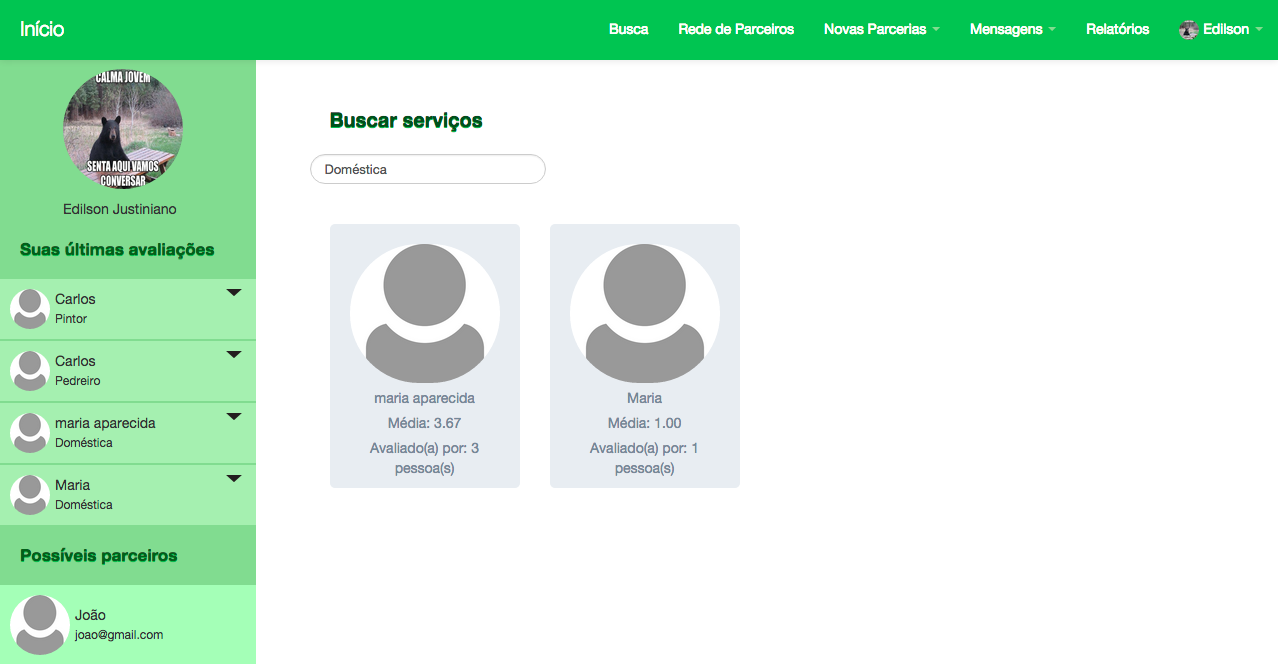
\includegraphics[scale=0.3]{./imagens/busca-domestica-edilson.png}}
	\caption[\textit Página resultante da busca por doméstica.]
	{\textit Página resultante da busca por doméstica \textbf{Fonte:} Elaborado pelos autores.}
	\label{fig:busca_domestica_edilson}
\end{figure}

\par A ideia desta funcionalidade foi apresentar um possível prestador de serviços que já tenha sido avaliado por alguém em comum ao usuário solicitante, desta forma, há uma confiança maior em relação ao profissional que está sendo contratado.
